\documentclass[11pt]{report}

\usepackage[utf8]{inputenc}
\usepackage{tikz}
\usepackage{minted}
\usepackage{geometry}
\usepackage{titlesec}
\usepackage{etoolbox}
\usepackage{indentfirst}

\usepackage{titlesec}
\titleformat{\chapter}[display]{\normalfont\huge\bfseries}{}{0pt}{\Huge}
\titleformat{\section}{\normalfont\Large\bfseries}{}{0pt}{}
\titleformat{\subsection}{\normalfont\bfseries}{}{0pt}{}
\titleformat{\subsubsection}{\normalfont\small\bfseries}{}{0pt}{}
\titlespacing*{\chapter} {0pt}{20pt}{40pt}

\geometry{
    a4paper,
    total={170mm, 257mm},
    left=20mm,
    top=20mm,
}

\title{\textbf{Computer Networks}}

\author{
    \Large
    Eduardo Correia \\
    \texttt{up201806433@fe.up.pt}
    \and
    \Large
    Ana Inês Barros \\
    \texttt{up201806593@fe.up.pt}
}

\date{\today}

\makeatletter
\renewcommand{\maketitle}{
    \begin{titlepage}
        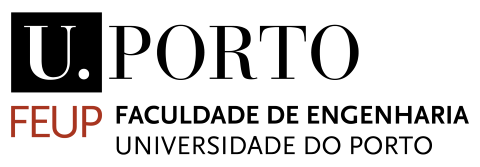
\includegraphics[width=0.5\textwidth]{images/feup.png}
        \begin{center} 
            \par\vspace{8cm}
            {\Huge\@title}
            \par\vspace{1cm}
            {\huge RCOM - Second Project}
            \par\vspace{1cm}
            \begin{tabular}[t]{c}
             \@author
            \end{tabular}
            \vfill
            \@date
        \end{center}
    \end{titlepage}
}
\makeatother

\begin{document}

\maketitle

\titlespacing*{\chapter}{0pt}{0pt}{1pt}

\tableofcontents

\chapter{Introduction}

This report was elaborated for the Computer Networks (RCOM) and it serves as a complement for the course unit's second project.

This project consisted in two different parts: the development of a download application according to the FTP protocol and the configuration and study of a computer network, using Cisco Router/Switch, which would then be used to test our download application.

\chapter{Part 1 - Development of a download application}

For this project, it was asked that we developed an application which downloaded a single file, implemented FTP application protocol, as described in RFC959 and adopts URL syntax, as described in RFC1738.

\section{Architecture}
We had to program the client side of the communication with the FTP server. Both implementing the TCP client - Transport layer and the FTP application - Application layer. To explain the architecture, we will explain the code step by step:
\begin{enumerate}
    \item URL Parsing 
    \item Communication with FTP server
    \item File Download
\end{enumerate}

\subsection{URL Parsing}

The program receives an URL of this syntax: \mintinline{c}{ftp://[<user>:<password>@]<host>/<url-path>}, as described in RFC1738.
In order to get the information from the URL, we use \mintinline{c}{int parse_url(char* arguments, struct url* url);} to parse the URL and the following struct to store the contents.

\begin{minted}{c}
    struct url {
        char user[50];
        char password[50];
        char filepath[100];
        char host[50];
    };
\end{minted}

\subsection{Communication with FTP server}
\subsubsection{Control Socket}
TCP use port numbers to identify sending and receiving application end-points on a host, often called Internet sockets. Using the host received in the URL, we are able to get an IP address. The port is 21 by default, since it is a well-known port. With this information we can open a socket and establish the connection in the transport layer.

\begin{minted}{c}
    #define SERVER_PORT 21
    #define h_addr h_addr_list[0] // The first address in h_addr_list.
    
    struct hostent* h = gethostbyname(url.host);
    char* address = inet_ntoa(*((struct in_addr*) h->h_addr)); // Get IP
\end{minted}

\newpage

\subsubsection{Communication}

The rest of the communication with the server is made with reads and writes to the socket file descriptor. Based on the code number of the messages, we verify if errors occurred or if we need to send a command. Here is an example of the login where we only send the password if needed: 

\textbf{Login:}
\begin{minted}{c}
    // Send User
    char buf[MAX_LEN];
    sprintf(buf, "user %s\n", url.user);
    write(sockfd, buf, strlen(buf);
    
    char res = readFromSocket(fp);
    //"331 Please specify the password".
    if (res == '3') {
        sprintf(buf, "pass %s\n", url.password);
        write(sockfd, buf, strlen(buf);
    }
\end{minted}

\subsubsection{File Download}

To download the file we send the "pasv" command to enter the passive mode. The server's reply will be made of a few numbers which we can use to calculate the new port. With this new port we are able to connect another socket, the data socket from where we will receive the file we want to download. After sending "retr name\_of\_file" command to the control socket, if the file exists, we start reading the file data from the data socket and writing into a file using the following function. 

\mintinline{c}{int download_file(int file_size, int data_socket_fd, char* filepath) }

\newpage

\section{Download Example}

\begin{figure}[h!]
    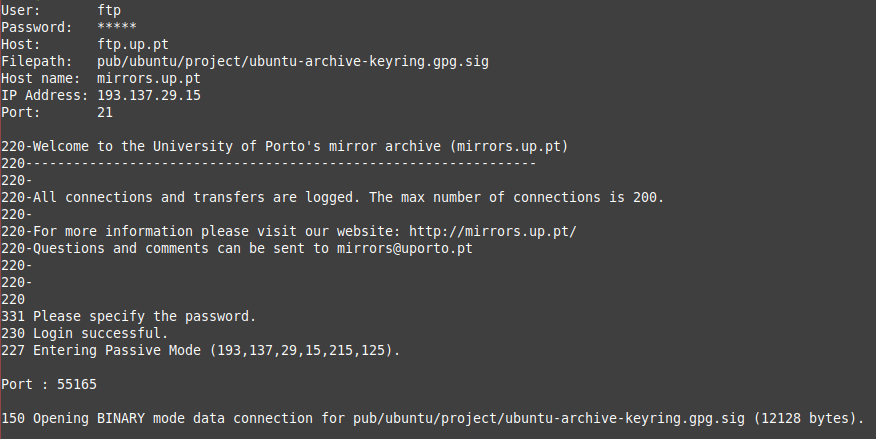
\includegraphics[width=10cm]{images/download_example.png}
\end{figure}

\begin{figure}[h!]
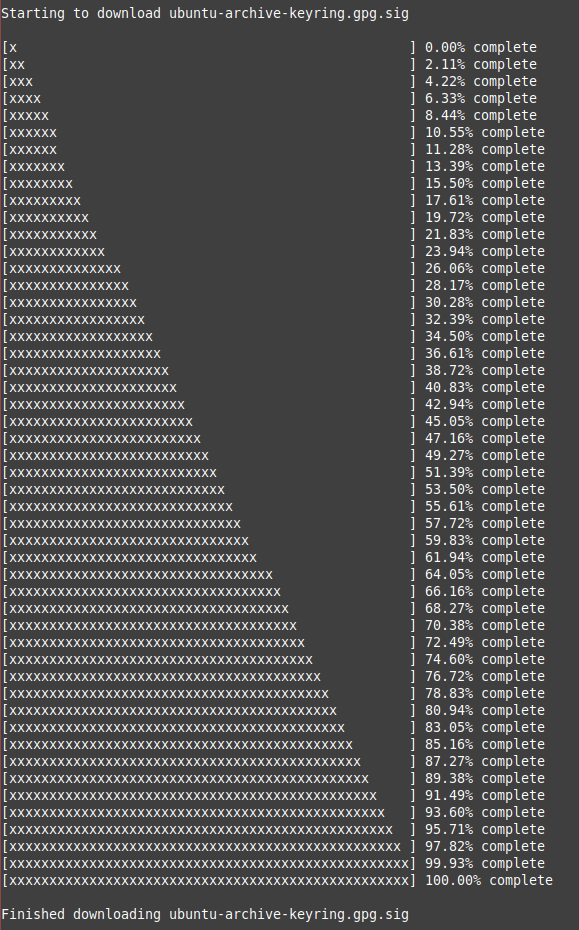
\includegraphics[width=10cm]{images/download_example2.png}
\end{figure}

\chapter{Part 2 - Configuration and Study of a Computer Network}

\section{Experience 1 - Configure an IP Network}

\subsection{What are the ARP packets and what are they used for?}

ARP packets are packets used in the \textit{Address Resolution Protocol}. These packets are used for discovering the link layer address associated with a given internet layer address, typically an IPv4 address.

\subsection{What are the MAC and IP addresses of ARP packets and why?}

ARP packets have the MAC and IP addresses of both the source and the target. When the target's MAC address is unknown, the source sends an ARP packet with the target's MAC address full of zeros (00:00:00:00:00:00). 

\textit{Consult figures \ref{fig:experience1_1} and \ref{fig:experience1_2}}

\subsection{What packets does the ping command generate?}

The ping command generates ARP packets first if target's MAC address is unknown. After finding out what the target's MAC address is, it generates ICMP packets.

\subsection{What are the MAC and IP addresses of the ping packets?}

The MAC and IP addresses of the ping packets are from the source and from the target.

\subsubsection{Request packet} 

\textit{Consult figure \ref{fig:experience1_3}}

\begin{itemize}
    \item \textbf{Packet source MAC address:} 00:21:5a:5a:78:c7 (tux3)
    \item \textbf{Packet destination MAC address:} 00:22:64:a7:26:a2 (tux4)
    \item \textbf{Packet source IP address:} 172.16.20.1 (tux3)
    \item \textbf{Packet destination IP address:} 172.16.20.254 (tux4)
\end{itemize}

\subsubsection{Reply packet}

\textit{Consult figure \ref{fig:experience1_4}}

\begin{itemize}
    \item \textbf{Packet source MAC address:} 00:22:64:a7:26:a2 (tux4)
    \item \textbf{Packet destination MAC address:}  00:21:5a:5a:78:c7 (tux3)
    \item \textbf{Packet source IP address:} 172.16.20.254 (tux4)
    \item \textbf{Packet destination IP address:} 172.16.20.1 (tux3)
\end{itemize}

\subsection{How to determine if a receiving Ethernet frame is ARP, IP, ICMP?}

By analyzing the Ethernet header of the frame. If the \textit{EtherType} has the value 0x800, we have an IP type frame. Being an IP type frame, if the IP header has value 1, it means it is a ICMP type frame. Otherwise, if the EtherType of the frame has value 0x806, it is a ARP type frame.

\textit{Consult figures \ref{fig:experience1_5} and \ref{fig:experience1_6}}

\subsection{How to determine the length of a receiving frame?}

By analyzing the third and fourth octets of the Ethernet header of a frame we can determine the length of a receiving frame.

\textit{Consult figure \ref{fig:experience1_7}}

\subsection{What is the loopback interface and why is it important?}

The loopback interface is a virtual interface which makes it possible for a source to receive answers from itself. It is useful for troubleshooting purposes.

\textit{Consult figure \ref{fig:experience1_8}}

\newpage

\section{Experience 2 - Implement Two Virtual LANs in a Switch}

\subsection{How to configure vlany0?}
Firstly, to configure vlany0 we have to connect the S0 port from tux4 to CISCO and we have to connect CISCO to the switch console. Then, we have to open GTKTerm on tux4 we login. Finally, to create the vlan we have to type the following commands, replacing 'y' by the number we want. In our case, it was 2.

\begin{minted}{sh}
    configure terminal
    vlan y0
    end
\end{minted}

To configure the vlan ports, we have to first connect the eth0 ports of the tux2, tux3 and tux4 to one of the ports of switch. We connect tux2's eth0 to switch's port 2, tux3's eth0 to switch's port 3 and tux4's eth0 to switch's port 4. After, we wait for a green light to appear next to the ports, this means the cable is correctly connected. Then, after taking note of the number of ports we connected, we run the following commands and replace the n with the number of the ports:

\begin{minted}{sh}
    configure terminal
    interface fastethernet 0/n
    switchport mode access
    switchport access vlan y0
    end
\end{minted}

\subsection{How many broadcast domains are there? How can you conclude it from
the logs?}

From the logs we conclude there are 2 broadcast domains: one for tux2 and another one for tux3 and 4. Since tux2 can not ping neither tux3 nor tux4, and tux3 and 4 can ping each other but not tux2. 

\newpage

\section{Experience 3 - Configure a Router in Linux}

\subsection{What routes are there in the tuxes? What are their meaning?}
\begin{figure}[h!]
    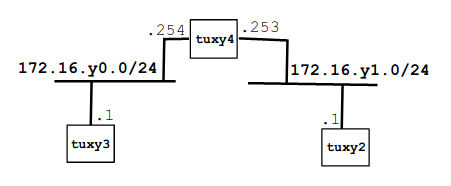
\includegraphics[width=7cm]{images/exp3 rotas.png}
\end{figure}
    
destination - gateway - interface

\subsubsection{Tux2 routes}

\begin{itemize}
    \item 172.16.20.0 - 172.16.20.253 - eth0
    \item 172.16.21.0 - 0.0.0.0 - eth0
\end{itemize}

\subsubsection{Tux3 sub routes}

\begin{itemize}
    \item 172.16.21.0 - 172.16.20.254 - eth0
    \item 172.16.20.0 - 0.0.0.0 - eth0
\end{itemize}

\subsubsection{Tux4 routes}

\begin{itemize}
    \item 172.16.20.254 - 0.0.0.0 - eth0
    \item 172.16.21.253 - 0.0.0.0 - eth1
\end{itemize}

By analyzing the routes, we can see that for tux3 to ping tux2, it uses tux4 as a gateway. Tux2 also uses tux4 to ping tux3.    

\subsection{What information does an entry of the forwarding table contain?}

\begin{itemize}
    \item \textbf{Destination:} IP address of the route's destination.
    \item \textbf{Gateway:} IP address of the gateway through which the network can be reached.
    \item \textbf{Netmask:} 32-bit mask used to determine the network's ID given the IP address of the route's destination.
    \item \textbf{Flags:} Information about the route.
    \item \textbf{Metric:} Cost of each route.
    \item \textbf{Ref:} Number of references to this route.
    \item \textbf{Use: } Route search counter.
    \item \textbf{Interface: } Network card (eth0/eth1) responsible for the gateway.
\end{itemize}

\subsection{What ARP messages, and associated MAC addresses, are observed and
why?}

An exchange of ARP messages occurs, when a computer sends a pings to another and it doesn't know the MAC address of the destination computer.

An ARP message is sent, in which the MAC address of the target is requested, given its IP address. 

\textit{Consult figure \ref{fig:experience3_1}}

When a ARP message is sent, the computer who's sending it, associates its MAC address to the message, so that the expected receiver of the message knows which computer to reply to.

This message is sent in broadcast mode (that is, the value of the receiver MAC address is 00:00:00:00:00:00), since the target MAC address is unknown. 

When the destination computer receives this broadcast message, it responds with an ARP message, in which is provided its MAC address. This message is sent only to the MAC address of the computer who sent the original message, instead of broadcast mode as well.

\textit{Consult figure \ref{fig:experience3_2}}

\subsection{What ICMP packets are observed and why?}

ICMP packets of type \texttt{Request} and \texttt{Reply} are observed, since, all routes being added, every computer recognizes the presence of the others. 

Otherwise, the ICMP packets sent would be of type \texttt{Host Unreachable}.

\subsection{What are the IP and MAC addresses associated to ICMP packets and
why?}

The IP and MAC addresses of origin and destination associated with the ICMP packets are the addresses of the computers/interfaces that receive/send packets..

For example, when a ICMP packet is sent from tux3 to tuxy4's interface connected to the same sub network (in this case, the interface eth0).

The origin IP and MAC addresses would be the same as tux3 (\textbf{IP address:} 172.16.20.1 and \textbf{MAC address:} 00:21:5a:78:c7) and the destination IP and MAC addresses would be the same as tux4 (\textbf{IP address:} 172.16.20.254 and \textbf{MAC address:} 00:22:64:a7:26:a2).

If the two computers weren't connected to the save virtual network (as it is the case of tux3 and tux2), it wouldn't be possible to exchange information between these two with just a ICMP packet without it being modified.

What would happen, in this case, is that tux3 would send a ICMP packet to tux4's eth0 interface, since this computer is connected to both virtual networks and is, therefore, able to interact directly with tux2. 

The IP addresses of this packet would correspond to tux3 (origin) and tux2 (destination) and the MAC addresses would correspond to tux3 and tux4's eth0 interface.

Upon receiving this packet, tux4 would forward it to tux2, keeping the IP addresses of the packet, but changing the associated MAC addresses so that the origin address would be of tux4 eth1's interface and that the destination address would be the MAC address of tux2 .

\newpage

\section{Experience 4 - Configure a Commercial Router and Implement NAT}

In this experience, we configured a commercial router, initially without NAT, connecting it to the laboratory network, and afterwards with NAT, thus allowing the access of the computers to the internet (however, only with direct IP address access, since the computers couldn't resolve hostnames yet).

\subsection{How to configure a static route in a commercial router?}

To configure the router we had to swap the Switch console port with the Router console port. After logging in we can run the following command in GTKTerm: 

\mintinline{sh}{ip route prefix mask {ip-address| interface-typeinterface-number[ip-address]} }

\subsection{What are the paths followed by the packets in the experiments carried out and why?}

If that path / route is defined, the packets will follow that route, otherwise, they will follow the default route that was defined. 

\subsection{How to configure NAT in a commercial router?}

Running the following commands in GTKTerm while connected to the router console.

\begin{minted}{sh}
conf t 
interface gigabitethernet 0/0  
ip address 172.16.y1.254 255.255.255.0 
no shutdown 
ip nat inside 
exit 

interface gigabitethernet 0/1 
ip address 172.16.1.y9 255.255.255.0 
no shutdown 
ip nat outside 
exit 

ip nat pool ovrld 172.16.1.y9 172.16.1.y9 prefix 24 
ip nat inside source list 1 pool ovrld overload 

access-list 1 permit 172.16.y0.0 0.0.0.7 
access-list 1 permit 172.16.y1.0 0.0.0.7 

ip route 0.0.0.0 0.0.0.0 172.16.1.254 
ip route 172.16.y0.0 255.255.255.0 172.16.y1.253 

end
\end{minted}

\subsection{What does NAT do?}

NAT stands for Network Address Translation and it is an IP translation tool. With NAT, private IP networks that use non-registered IPs are able to connect to the Internet and the public network. NAT operates in a router where 2 networks are connected and the private IPs are translated to public IPs. In other words, it makes it possible for computers that belong to a private network to be represented by only one public IP outside their network. NAT is also used for security reasons. 

\newpage

\section{Experience 5 - DNS}

In this experience, it was necessary to configure the DNS (Domain Name System).

A DNS server, in this case, \texttt{services.netlab.fe.up.pt}, contains a database of the public IP address and their respective \textit{hostnames} and it's used to translate between these two.

\subsection{How to configure the DNS service at an host?}

To configure the DNS service, it was necessary to change the file \texttt{resolve.conf}, a file used in Linux (and various operating systems) to configure the system's DNS resolver.

It was located in the folder \texttt{/etc/} of the computer host and the following 2 lines were written to the file:

\begin{minted}{sh}
    search netlab.fe.up.pt 
    nameserver 172.16.1.1
\end{minted}

In this case, \texttt{netlab.fe.up.pt} corresponds to the DNS server hostname and 172.16.1.1 is its IP address.

After this experience, it's possible to access the internet, since the computer is now able to solve hostnames such as \texttt{google.com}.

\subsection{What packets are exchanged by DNS and what information is transported?}

The host starts by sending a packet to the server, containing the desired hostname whose IP address is being asked to know.
The server then answers with a packet containing the hostname's corresponding IP address.

\newpage

\section{Experience 6 - TCP Connections}

In this final experience, we put our FTP application download and network configuration to the test, culminating all of our work developed up to this point.

\subsection{How many TCP connections are opened by your FTP application?}

The FTP application opened two TCP connections: one to send and receive the FTP commands to and from the server and another one to receive the data we're downloading sent by server.

\subsection{In what connection is transported the FTP control information?}

The FTP control information is transported in the TCP connection responsible for the command exchange.

\subsection{What are the phases of a TCP connection?}

A TCP connection can split in essentially three phases:

\begin{enumerate}
    \item Connection establishment
    \item Data exchange
    \item Connection shutdown
\end{enumerate}

\subsection{How does the ARQ TCP mechanism work? What are the relevant TCP
fields? What relevant information can be observed in the logs?}

TCP (Transmission Control Protocol) uses ARQ (Automatic Repeat Request/Query) with the sliding window mechanism, that consists in the error control of the data transmission. This mechanism uses acknowledgements and timeouts in order to ensure a secure connection. 
For that purpose, it utilizes \textit{acknowledgment numbers}, that are present in a field of header of the messages sent by the receiver. These also denote that the frame was received correctly, the range of packets that the transmitter can send (window size) and the sequence number, the packet number to be send.

\begin{figure}[h!]
    \centering
    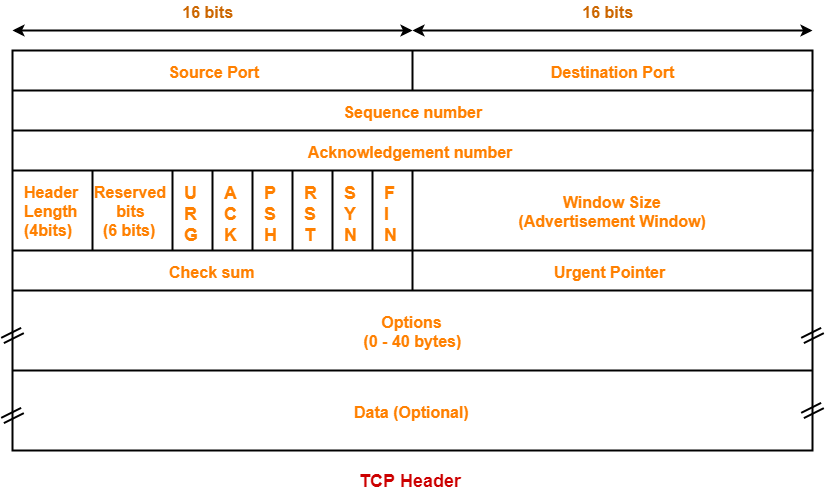
\includegraphics[width=0.8\textwidth]{images/TCP_Header_Format.png}
\end{figure}

\subsection{How does the TCP congestion control mechanism work? What are the
relevant fields. How did the throughput of the data connection evolve
along the time? Is it according the TCP congestion control mechanism?}

The TCP congestion control relies on a congestion window based on the octets number that the network is able to forward and not sending more octets than the minimum defined by both the receiver and the congestion window.

When analyzing the data connection, we noticed that whenever the network was more congested, the bit rate would be lower that when it was less congested. This behaviour was expected since it goes along with what we explained before.

\textit{Consult figure \ref{fig:experience6_1}}

\subsection{Is the throughput of a TCP data connections disturbed by the appearance of a second TCP connection? How?}

Yes, it is possible. With the emergence of a second TCP connection, the simultaneous existence of a data transference can lead to a fall in the baud rate, since the transfer rate is equally distributed by each connection.

\chapter{Conclusion}

Concluding, we believe that all of the main goals of this project were achieved and that we consolidated and absorbed new concepts about computer networks, deepening our knowledge about this area that surrounds each day with the ever growing inter connectivity of our devices.

This project had a special impact on us for one particular reason, since it was the first time we got to really have contact with a more practical approach inside a laboratory, in a course that's mainly theoretical.

However, given the situation we're living in, increased difficulties were raised. Due to the access to the laboratories being restricted and four days of classes being cancelled (due to holidays), we struggled to work on the project. 
However, we managed to perform every experience successfully in the end.

\section{Note about number of pages}
We're aware that it was requested to keep the number of pages of this report up to a maximum of eight. However, we wanted to include the necessary information and illustrations, while still maintaining the content spaced out and structured to allow for easier readability. 
We hope that the professor understands.

\chapter{Attachments}

\section{Experience 1}

\begin{figure}[h!]
    \centering
    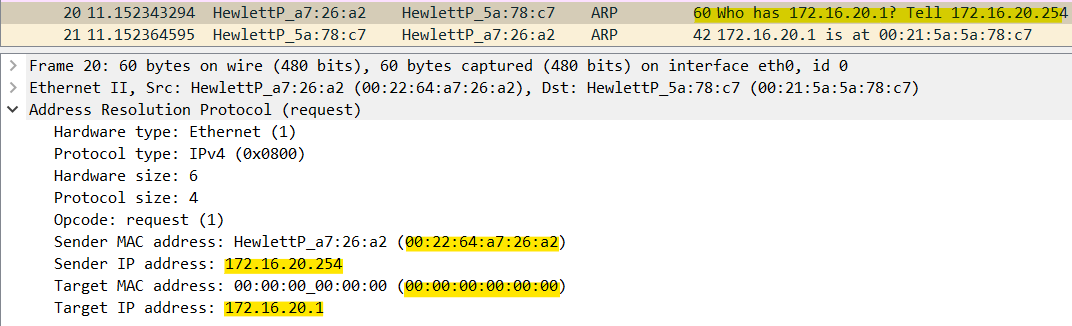
\includegraphics[width=\textwidth]{images/Experience1_1.png}
    \caption{}
    \label{fig:experience1_1}
\end{figure}

\begin{figure}[h!]
    \centering
    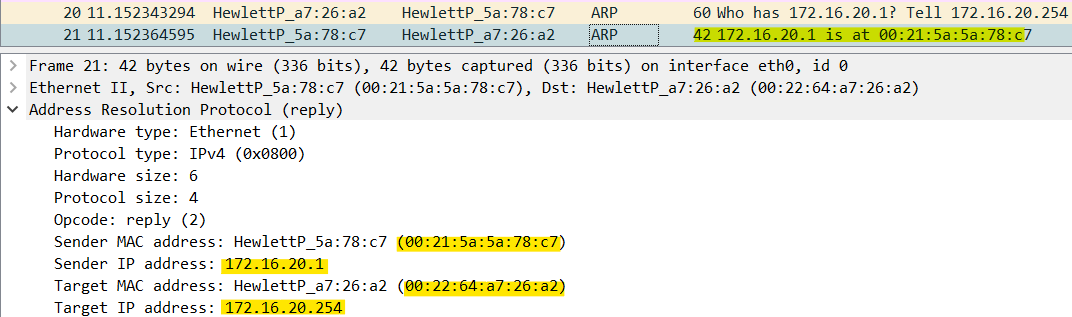
\includegraphics[width=\textwidth]{images/Experience1_2.png}
    \caption{}
    \label{fig:experience1_2}
\end{figure}

\begin{figure}[h!]
    \centering
    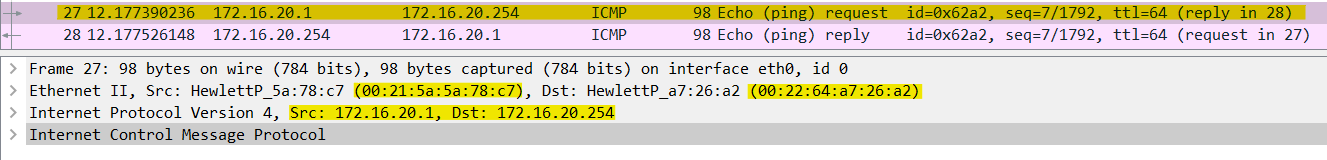
\includegraphics[width=\textwidth]{images/Experience1_3.png}
    \caption{}
    \label{fig:experience1_3}
\end{figure}

\begin{figure}[h!]
    \centering
    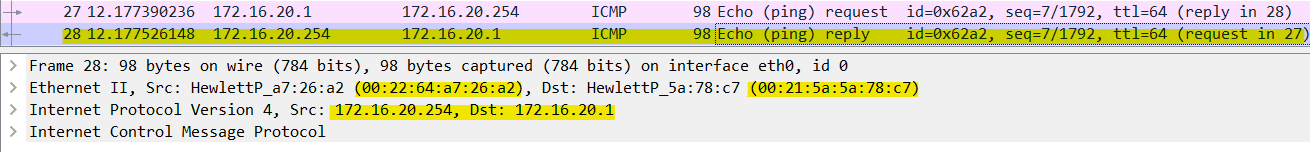
\includegraphics[width=\textwidth]{images/Experience1_4.png}
    \caption{}
    \label{fig:experience1_4}
\end{figure}

\begin{figure}[h!]
    \centering
    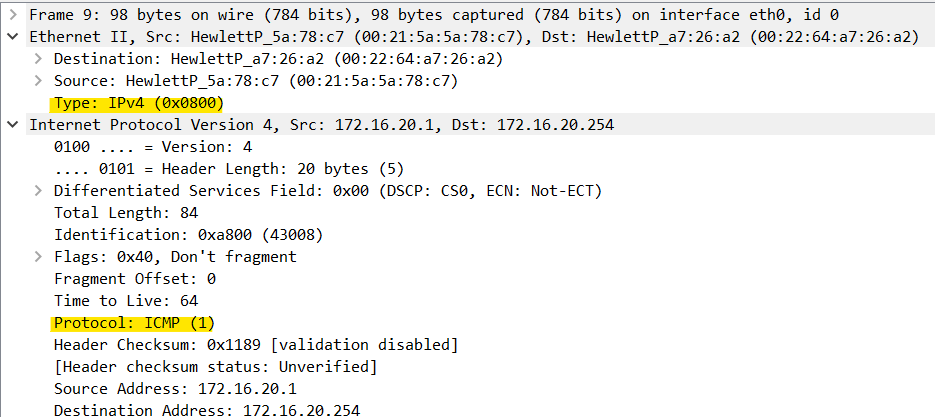
\includegraphics[width=\textwidth]{images/Experience1_5.png}
    \caption{}
    \label{fig:experience1_5}
\end{figure}

\begin{figure}[h!]
    \centering
    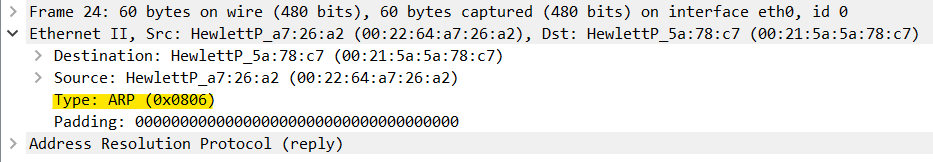
\includegraphics[width=\textwidth]{images/Experience1_6.png}
    \caption{}
    \label{fig:experience1_6}
\end{figure}

\begin{figure}[h!]
    \centering
    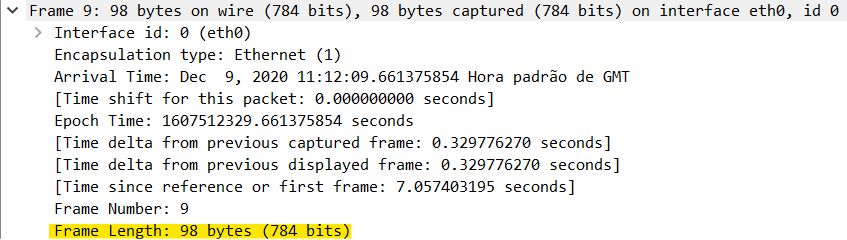
\includegraphics[width=\textwidth]{images/Experience1_7.png}
    \caption{}
    \label{fig:experience1_7}
\end{figure}

\begin{figure}[h!]
    \centering
    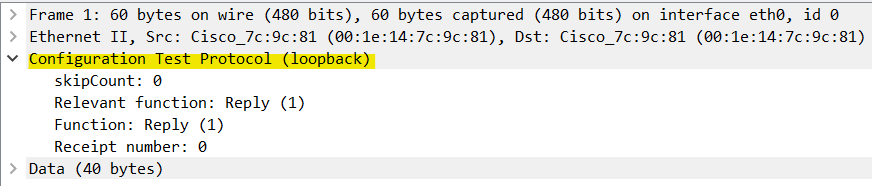
\includegraphics[width=\textwidth]{images/Experience1_8.png}
    \caption{}
    \label{fig:experience1_8}
\end{figure}

\clearpage

\section{Experience 3}

\begin{figure}[h!]
    \centering
    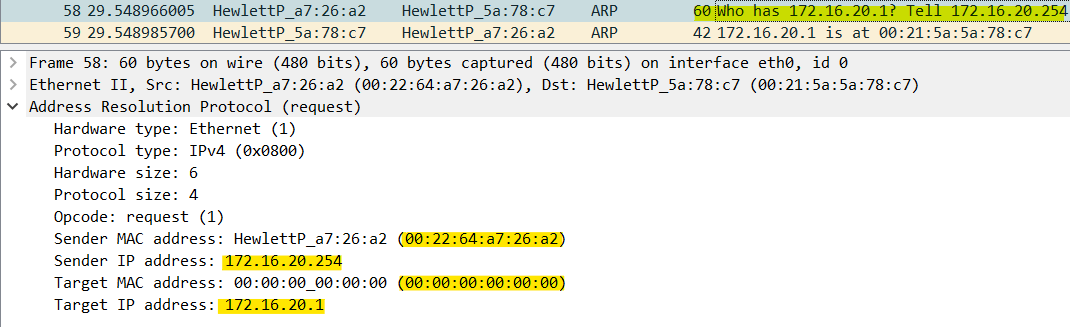
\includegraphics[width=\textwidth]{images/Experience3_1.png}
    \caption{}
    \label{fig:experience3_1}
\end{figure}

\begin{figure}[h!]
    \centering
    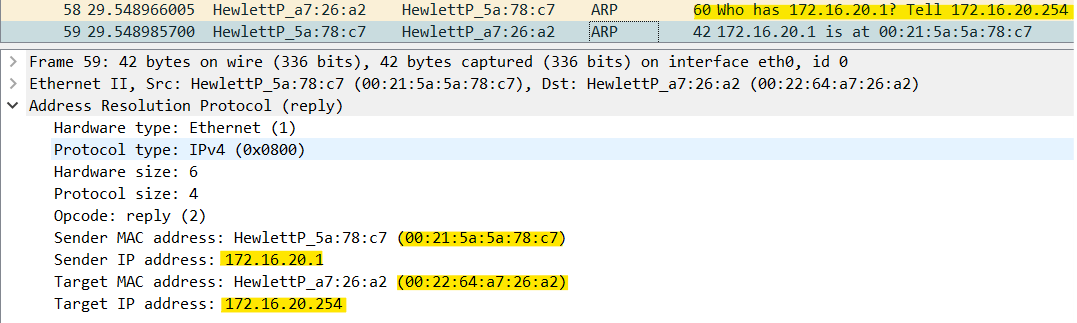
\includegraphics[width=\textwidth]{images/Experience3_2.png}
    \caption{}
    \label{fig:experience3_2}
\end{figure}

\clearpage

\section{Experience 6}

\begin{figure}[h!]
    \centering
    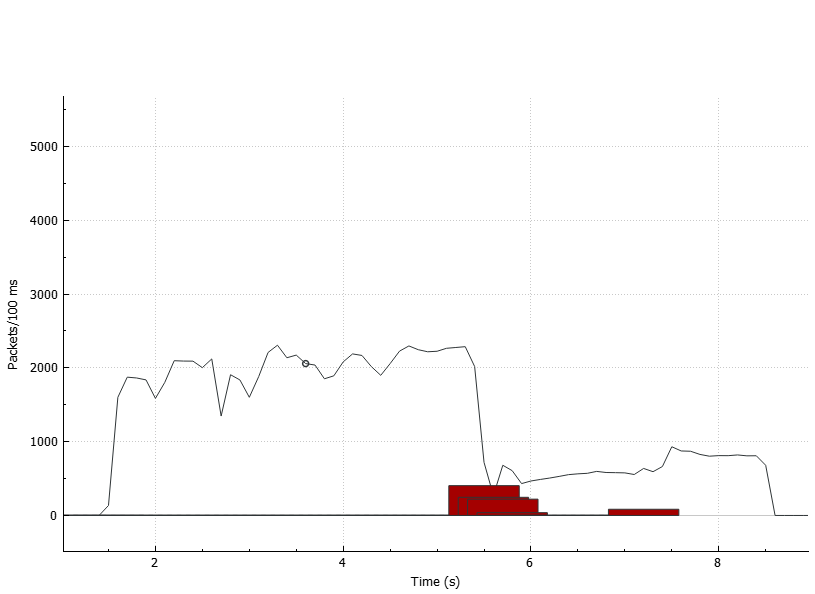
\includegraphics[width=\textwidth]{images/Experience6_1.png}
    \caption{}
    \label{fig:experience6_1}
\end{figure}

\clearpage

\section{FTP Client Application}

\subsection{download.c}

\inputminted[breaklines]{c}{../src/download.c}

\newpage

\subsection{utils.c}

\inputminted[breaklines]{c}{../src/utils.c}

\newpage

\subsection{utils.h}

\inputminted[breaklines]{c}{../src/utils.h}

\newpage

\subsection{Makefile}

\inputminted[breaklines]{make}{../src/Makefile}

\end{document}